\documentclass[runningheads]{llncs}
\usepackage{amsmath,amssymb}
\usepackage{graphicx}
\usepackage{booktabs}
\usepackage{multirow}
\usepackage{url}
\usepackage{hyperref}
\usepackage{xcolor}
\usepackage{ctex}

\begin{document}

\title{IntentAgent：面向检索增强生成的意图感知渐进式智能检索}

\author{作者姓名}
\institute{机构名称}

\maketitle

\begin{abstract}
检索增强生成（RAG）系统在面对多样化的查询意图时，现有方法普遍采用统一的检索策略，忽视了查询意图对检索路径选择的决定性影响。本文提出 IntentAgent，一种面向 RAG 的意图感知渐进式智能检索框架，核心命题是将查询意图作为检索策略选择的一等公民。IntentAgent 沿可控性-自适应性谱系设计三阶段渐进演化：（1）意图分类与静态路由——定义六类查询意图（事实性、分析性、比较性、多跳性、探索性、跟进性），构建级联 LLM 与正则表达式回退的双路径分类器，并通过确定性映射表将意图标签路由至差异化检索策略；（2）动态工具编排——将检索过程建模为五节点循环有向状态图，LLM 按推理-动作协议自主选择并组合检索工具，配合双模反思机制（启发式评分与 LLM 语义批评）和策略回退阶梯实现 Reflexion 式自纠正，CrossEncoder 重排序器提供语义级结果优化；（3）经验记忆增强——按意图分桶的持久化存储遵循召回-注入-持久化闭环，失败教训优先采用语义反思文本，赋予系统跨会话自我改进能力。在 HotpotQA、2WikiMultiHopQA 和 MuSiQue 上对 Gemma4-12B、Qwen3-8B 和 Qwen3-32B 骨干模型的实验表明，IntentAgent 与最强基线 HippoRAG2 取得极具竞争力的性能，并显著优于其余基于文本、基于图和混合检索方法。消融研究证实，意图分类是核心贡献组件（移除后 EM 下降 10.4\%--15.6\%），动态编排与反思循环次之。在忠实度和答案相关性上，IntentAgent 均取得最优，验证了意图感知检索在减少幻觉和提升语义相关性方面的显著优势。

\noindent\textit{关键词：}检索增强生成，意图感知检索，经验记忆，智能体
\end{abstract}

\section{引言}

检索增强生成（RAG）在推理时通过外部知识检索来增强大语言模型，已成为缓解幻觉和提高事实准确性的主流范式~\cite{ref1}。典型的 RAG 系统遵循检索-阅读-生成流程：给定用户查询，首先从知识库中检索相关段落，然后将其作为上下文提供给 LLM 以生成答案~\cite{ref2}。

然而，现有 RAG 系统在检索阶段共享一个隐含且限制性的假设，我们称之为\emph{策略同质性假设}：无论查询意图如何，系统都应用相同的检索流程——通常是单次向量相似度搜索。这一假设在面对现实世界查询多样性时失效。考虑三种代表性查询类型。诸如"谁发明了万维网？"的事实性查询仅需单次向量检索即可定位答案段落。诸如"爱因斯坦的母校对量子力学的发展有何影响？"的多跳推理查询需要跨多个实体的桥接推理，单次检索很难覆盖完整的证据链。诸如"比较 BERT 和 GPT 在文本分类任务上的性能"的比较性查询需要并行检索两个实体的信息，然后进行结构化比较。

这三种查询类型的最优检索路径差异显著。将多跳推理查询路由到单次向量检索流程往往导致证据不完整或缺失，而对简单事实性查询应用复杂的多跳策略则引入不必要的延迟和计算开销。

\begin{figure*}[htbp]
\centering
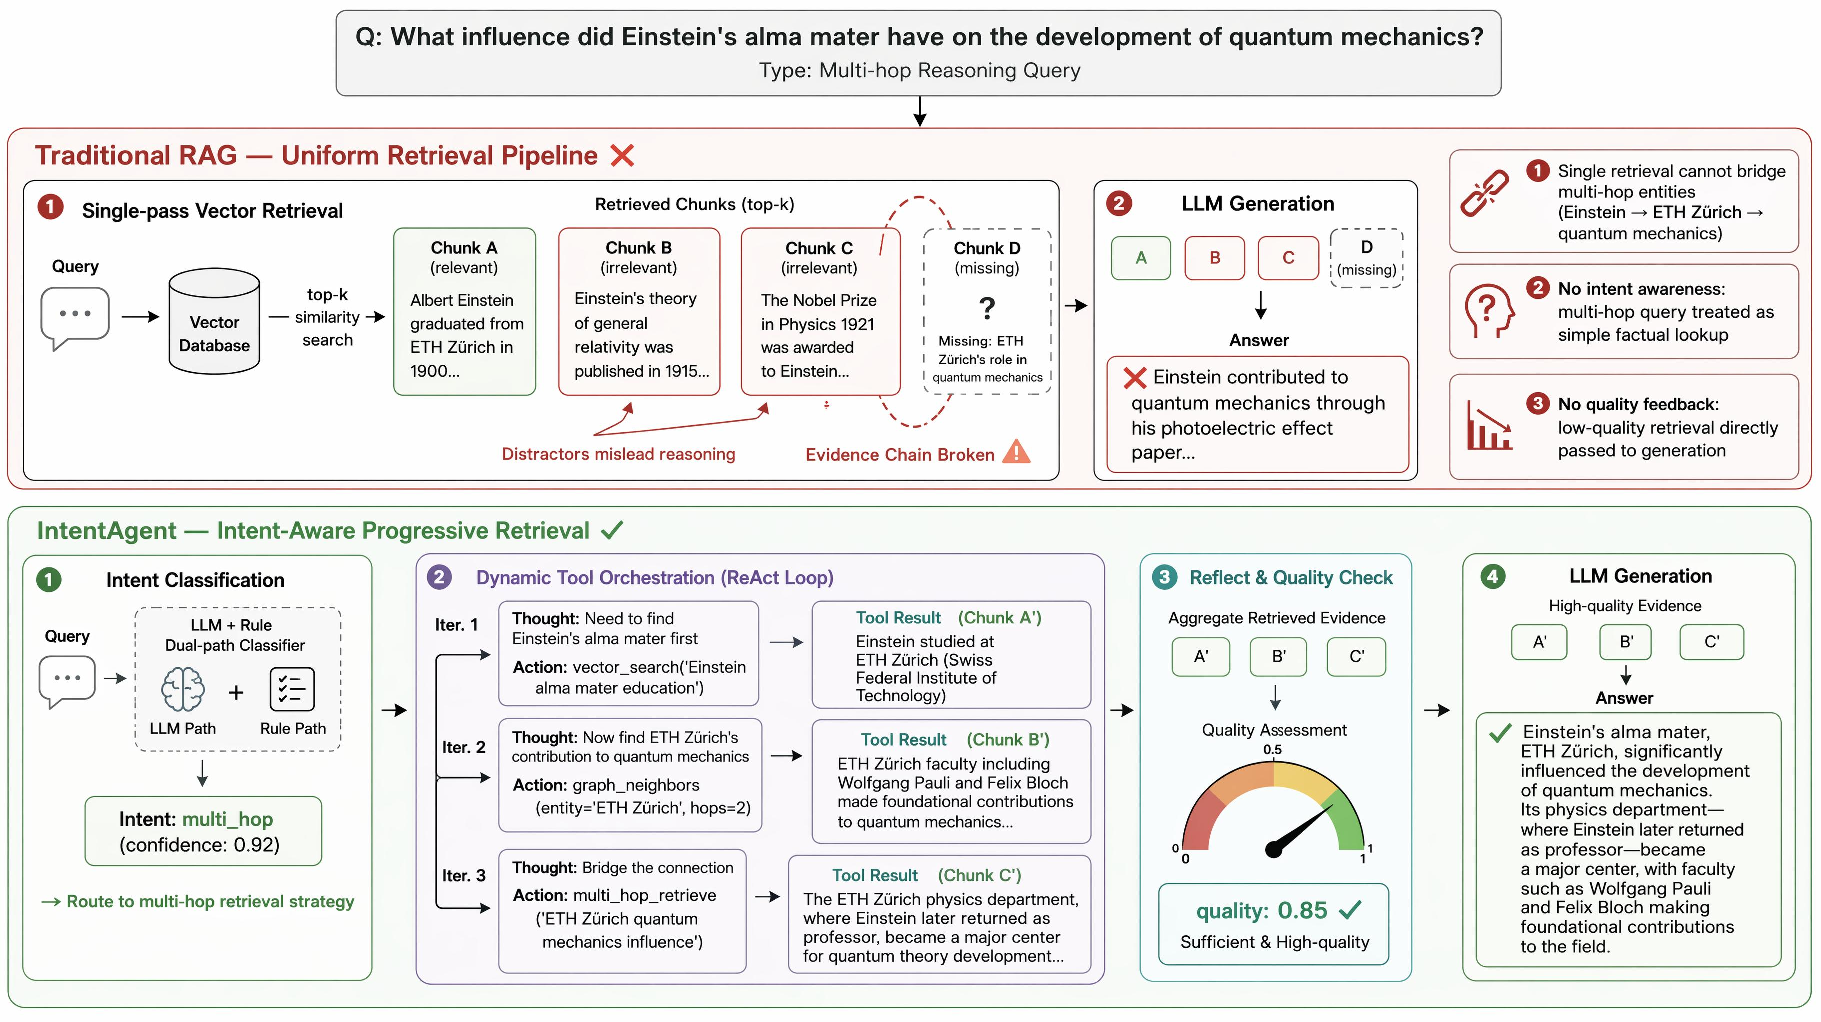
\includegraphics[width=\textwidth]{figures/figure1.pdf}
\caption{传统 RAG 与 IntentAgent 的对比。以多跳查询"爱因斯坦的母校对量子力学的发展有何影响？"为例，上半部分说明传统 RAG 因策略同质性而遭受证据链断裂和干扰项影响，下半部分展示 IntentAgent 如何通过意图感知渐进式检索组装完整的证据链。}
\label{fig:comparison}
\end{figure*}

尽管近年来涌现出多种检索机制层面的改进方法——包括基于层次化摘要树的 RAPTOR~\cite{ref23}、基于社区摘要的 GraphRAG~\cite{ref27}、基于双层检索的 LightRAG~\cite{ref26}、借鉴海马体索引机制的 HippoRAG~\cite{ref28} 和 HippoRAG2，以及直接在知识图谱上进行推理引导导航的 TOG~\cite{ref24}——这些方法在检索后端各有创新，但在策略选择层面均未解决策略同质性问题：检索策略由系统架构在部署时固化决定，对任意查询均触发相同的检索流程，查询意图对策略路由毫无影响。在此框架下，事实型查询因调用成本高昂的多跳图扩展而引入不必要的延迟；多跳推理查询因缺乏跨实体的图扩展而导致证据链断裂；比较性查询因缺乏并行子检索而只能获取单侧信息。问题的根源不在于检索机制本身，而在于策略选择逻辑对查询意图的漠视。意图感知的差异化路由是填补这一空白的关键缺失环节。

本文的核心命题是：查询意图应作为检索策略选择的一等公民。我们将这一命题实例化为 IntentAgent，其设计通过三阶段渐进演化在可控性和自适应性之间取得平衡。

在意图分类与静态路由中，我们定义六类查询意图分类（事实性、分析性、比较性、多跳性、探索性和跟进性），并设计一个级联 LLM 与基于规则回退的双路径分类器。分类结果通过确定性映射表路由到预定义的检索策略。

在动态工具编排中，我们解决静态路由无法处理跨意图查询和运行时自适应的问题。有向状态图将检索过程重构为 LLM 驱动的工具选择循环：LLM 按照推理-动作协议~\cite{ref13}自主决定调用哪些检索工具及其顺序，同时反思节点评估证据质量并在质量分数低于阈值时触发重新规划。

在经验记忆增强中，我们解决动态编排每次决策都从零开始的局限性。意图分桶的持久化经验存储实现召回-注入-持久化闭环，赋予系统跨会话自我改进能力。

我们在 HotpotQA~\cite{ref20}、2WikiMultiHopQA~\cite{ref21} 和 MuSiQue~\cite{ref22} 上对 Qwen3-8B 和 Qwen3-32B 骨干模型进行系统实验。结果表明，IntentAgent 在所有数据集和骨干配置下，相对于所有代表性基线（包括 Vanilla RAG、RAPTOR~\cite{ref23}、TOG~\cite{ref24}、G-Retriever~\cite{ref25}、LightRAG~\cite{ref26}、GraphRAG~\cite{ref27}、HippoRAG~\cite{ref28} 和 HippoRAG2）取得极具竞争力的性能，与最强基线 HippoRAG2 差距极小，并显著优于其余所有方法。

本文的主要贡献如下：（1）我们将查询意图建模为检索策略选择的主要依据，定义六类意图分类及相应的差异化检索策略族，将检索从统一匹配转变为意图驱动的分化。（2）我们提出从静态路由到动态编排再到经验记忆的三阶段渐进演化，每个阶段解决前一阶段的局限性，并沿可控性-自适应性谱系推进。（3）我们将检索过程公式化为具有决策-工具调用-反思循环的 LLM 驱动有向状态图，引入双模质量评估（启发式信号与 LLM 语义反思）和策略回退阶梯实现 Reflexion 式自纠正，使智能体能够自主组合多个检索原语并在质量不足时自动升级策略。（4）我们引入具有三阶段闭环的意图分桶持久化经验存储，失败教训优先采用 LLM 语义反思文本，实现跨会话自我改进，使相似查询的检索效果随使用积累而提升。

\section{相关工作}

\subsection{检索增强生成}

检索增强生成由 Lewis 等人~\cite{ref1}首次提出，将信息检索与序列到序列生成相结合，通过在推理时动态检索外部知识来增强语言模型输出。Borgeaud 等人~\cite{ref3}随后提出 RETRO，将检索机制深度集成到 Transformer 架构中。Gao 等人~\cite{ref2}对 RAG 技术栈进行系统综述，识别出三个演化阶段：朴素 RAG、高级 RAG 和模块化 RAG。

在检索策略层面，查询重写工作线通过重新表述用户查询来提高检索质量，代表性方法包括 HyDE~\cite{ref4} 和 Query2Doc~\cite{ref5}。多步检索工作线迭代累积证据，代表性方法包括 Self-RAG~\cite{ref6} 和 CRAG~\cite{ref7}。

在图增强检索方面，GraphRAG~\cite{ref27}使用社区结构对知识图谱进行层次化摘要。LightRAG~\cite{ref26}通过双层检索实现轻量级图增强检索。HippoRAG~\cite{ref28}借鉴海马体记忆索引理论。HippoRAG 2~\cite{ref30}在 HippoRAG 基础上引入稠密-稀疏融合的知识图谱结构、深度上下文化检索机制和识别记忆模块，在事实记忆、语义理解和关联性推理三个维度上取得全面提升，是目前多跳问答中性能最强的图增强检索方法之一。TOG~\cite{ref24}将 LLM 作为智能体进行知识图谱上的推理引导导航。G-Retriever~\cite{ref25}通过图神经网络执行联合检索。RAPTOR~\cite{ref23}通过递归聚类和摘要构建层次化检索树。

上述方法均未将查询意图作为检索策略选择的显式依据。IntentAgent 的关键区别在于它在\emph{检索开始之前}识别查询意图，并据此将查询路由到最合适的检索路径。

\subsection{意图识别与查询理解}

查询意图识别在信息检索和对话系统中有着悠久的研究历史。Broder~\cite{ref8}首次将网页搜索意图分为导航型、信息型和事务型，后续工作逐步细化了这一分类~\cite{ref9,ref10}。在对话系统中，意图识别通常作为自然语言理解模块的核心任务~\cite{ref11}。最近，LLM 的零样本和少样本分类能力为意图识别开辟了新途径~\cite{ref12}。

我们的意图分类与先前工作的关键区别在于：六类意图旨在区分检索策略而非建模用户目标。每个意图类别直接映射到特定检索策略的最优应用场景。

\subsection{基于智能体的检索与经验学习}

ReAct~\cite{ref13}提出交错推理和行动的范式。思维树~\cite{ref14}将搜索过程建模为树状探索。Toolformer~\cite{ref15}展示 LLM 自主学习 API 调用的能力。

在经验学习方面，Reflexion~\cite{ref16}提出基于语言反馈的强化学习范式。Voyager~\cite{ref17}实现自动技能库积累和复用。MemoRAG~\cite{ref18}探索将检索经验纳入长期记忆。

我们的工作在三方面推进了这一研究线：（1）将意图分类作为先验信息注入智能体；（2）显式反思循环提供质量门控；（3）意图分桶的经验存储实现跨会话学习。

\section{方法}

本节详述 IntentAgent 框架。我们首先形式化问题并定义核心组件（§3.1），然后提供系统概述（§3.2），随后三个小节分别描述意图分类与静态路由（§3.3）、动态工具编排（§3.4）和经验记忆增强（§3.5）。

\subsection{问题形式化}

给定由$N$个文档衍生的文本块组成的知识库$\mathcal{K} = \{d_1, d_2, \ldots, d_N\}$和从$\mathcal{K}$构建的知识图谱$\mathcal{G} = (\mathcal{V}, \mathcal{E})$，其中$\mathcal{V}$表示实体集，$\mathcal{E}$表示关系三元组集，用户提交查询$q$。RAG 系统的目标是检索证据集$\mathcal{R}(q) \subseteq \mathcal{K}$并生成以$\mathcal{R}(q)$为条件的答案$a$。

传统 RAG 系统采用固定检索函数$f_{\text{retrieve}}: q \mapsto \mathcal{R}(q)$，对所有查询应用相同的检索逻辑。我们认为最优检索函数应取决于查询的意图类型。形式上，我们定义意图分类函数$\phi: q \mapsto l \in \mathcal{L}$，其中$\mathcal{L} = \{\texttt{factual}, \texttt{analytical}, \texttt{comparative}, \texttt{multi\_hop}, \texttt{exploratory}, \texttt{follow\_up}\}$是六类意图标签集，以及策略族$\mathcal{S} = \{s_l\}_{l \in \mathcal{L}}$，其中每个$s_l$是针对意图$l$优化的检索函数。IntentAgent 的目标是：
\begin{equation}
    \mathcal{R}^*(q) = s_{\phi(q)}(q, \mathcal{K}, \mathcal{G})
\end{equation}
系统首先识别查询意图，然后将查询路由到相应的最优策略。

\paragraph{双路径分类器。}
意图分类函数采用级联设计，包含 LLM 优先路径和基于规则的回退：
\begin{equation}
    \phi(q) = \begin{cases}
    (l_{\text{llm}}, c_{\text{llm}}) & \text{如果 } c_{\text{llm}} \geq \tau_c \wedge l_{\text{llm}} \in \mathcal{L} \\
    \phi_{\text{rule}}(q) & \text{否则}
    \end{cases}
\end{equation}
其中$(l_{\text{llm}}, c_{\text{llm}}) = \text{LLM}(q)$是 LLM 返回的意图标签和置信度，$\tau_c = 0.6$是置信度阈值。规则路径$\phi_{\text{rule}}$是优先级排序的正则表达式级联$\{(r_i, l_i, c_i)\}_{i=1}^{M}$：
\begin{equation}
    \phi_{\text{rule}}(q) = (l_j, c_j), \quad j = \min\{i \mid r_i \text{ 匹配 } q\}
\end{equation}
无规则匹配时返回默认值$(\texttt{factual}, 0.4)$。

\paragraph{意图-策略映射。}
意图标签通过确定性函数$\mathcal{M}: \mathcal{L} \to \mathcal{S}$映射到检索策略：
\begin{equation}
    \mathcal{M}(l) = \begin{cases}
    s_{\text{direct}} & l = \texttt{factual} \\
    s_{\text{iterative}} & l = \texttt{analytical} \\
    s_{\text{parallel}} & l = \texttt{comparative} \\
    s_{\text{multi\_hop}} & l = \texttt{multi\_hop} \\
    s_{\text{expansion}} & l = \texttt{exploratory} \\
    s_{\text{context}} & l = \texttt{follow\_up}
    \end{cases}
\end{equation}

\paragraph{检索工具集。}
检索原语被封装为五个结构化工具$\mathcal{T} = \{t_1, \ldots, t_5\}$，每个工具$t_i: \Theta_i \to \mathcal{R}_i$从参数空间映射到检索结果：$t_1$（向量检索）计算$t_1(q, k) = \text{top-}k\text{ nearest}(\text{embed}(q), \mathcal{K})$；$t_2$（图邻居扩展）返回$t_2(e, h) = \{(s, p, o) \in \mathcal{E} \mid \text{dist}(e, s) \leq h \vee \text{dist}(e, o) \leq h\}$；$t_3$（多跳检索）组合$t_3(q) = t_1(q, k) \cup t_2(\text{entities}(t_1(q, k)), h)$；$t_4$（并行检索）执行$t_4(q) = \bigcup_{i=1}^{m} t_1(q_i, k)$；$t_5$（证据评估）评估质量$t_5(q, \mathcal{C}) \to [0,1]^3$。跨工具证据累积由共享上下文$\mathcal{C}: \text{chunk\_id} \to \text{score}$协调：
\begin{equation}
    \mathcal{C}[c.\text{id}] \leftarrow \max(\mathcal{C}[c.\text{id}],\ \text{score}(c)), \quad \forall c \in t_i(\theta_i)
\end{equation}
合并输出为$\text{merge}(\mathcal{C}) = \text{sort\_desc}(\mathcal{C})[:k]$。

\paragraph{有向状态图。}
检索过程被建模为循环有向状态图$G_s = (V_s, E_s)$，具有五个节点$V_s = \{v_{\text{mem}}, v_{\text{reas}}, v_{\text{dec}}, v_{\text{tool}}, v_{\text{ref}}\}$和两条条件边。智能体状态定义为$\mathbf{S} = (q, l, \mathbf{m}, n, Q, \mathbf{T}_{\log})$。路由函数为：
\begin{equation}
    \text{route}_1(a) = \begin{cases}
    v_{\text{tool}} & \text{如果 } a = (\text{tool\_call}, t_i, \theta_i) \\
    v_{\text{ref}} & \text{否则}
    \end{cases}
\end{equation}
\begin{equation}
    \text{route}_2(Q, n) = \begin{cases}
    \text{END} & \text{如果 } Q \geq \tau \vee n \geq n_{\max} \\
    v_{\text{dec}} & \text{否则}
    \end{cases}
\end{equation}

\paragraph{质量评估与自反思。}
质量评估函数$\text{Eval}(q, a)$采用双模设计，从相关性$Q_{\text{relevance}}$和完整性$Q_{\text{completeness}}$两个维度评估答案质量，输出$Q_{\text{quality}} \in [0,1]$。Self-Reflection 模式下，当$Q < \tau$时，LLM 生成语义批评文本$\text{reflection\_text}$并注入下一轮决策消息序列。

\paragraph{策略回退阶梯。}
反思触发重新规划时，策略按证据收集能力递增自动升级：
\begin{equation}
    \text{direct} \to \text{multi\_hop} \to \text{iterative} \to \text{parallel} \to \text{expansion} \to \text{context\_aware}
\end{equation}

\paragraph{经验记忆。}
每条经验记录定义为$e = (l, q, \mathbf{T}_{\text{seq}}, n, Q_f, o, \lambda, a, \mathbf{E}, h, \text{ts})$，包含意图标签$l$、查询$q$、工具序列$\mathbf{T}_{\text{seq}}$、质量分数$Q_f$、类别$o \in \{\text{success}, \text{lesson}\}$等字段。条目分类为：
\begin{equation}
    o = \begin{cases}
    \text{success} & \text{如果 } Q_f \geq \tau \\
    \text{lesson} & \text{如果 } Q_f < \tau
    \end{cases}
\end{equation}
经验存储按意图分桶$\mathcal{B}_l$，遵循召回-注入-持久化闭环。召回函数为：
\begin{equation}
    \text{Recall}(l, N_r) = \text{top}_{N_r}\!\left(\mathcal{B}_l,\ \text{key} = (Q_f \downarrow,\ h \downarrow)\right)
\end{equation}
注入将召回条目渲染为系统消息$\mathbf{m}_{\text{exp}}$前置到初始状态。持久化提炼新条目$e_{\text{new}}$并写入$\mathcal{B}_l$，共享去重键$\kappa(e) = (\mathbf{T}_{\text{seq}}, o)$的条目执行合并更新。桶容量$C_{\max}$溢出时应用冷旧优先驱逐。

三阶段渐进演化体现在策略选择机制的日益复杂化：从确定性映射$\mathcal{M}(l)$到 LLM 驱动的动态选择再到经验增强的自适应决策。

\subsection{系统概述}

\begin{figure*}[htbp]
\centering
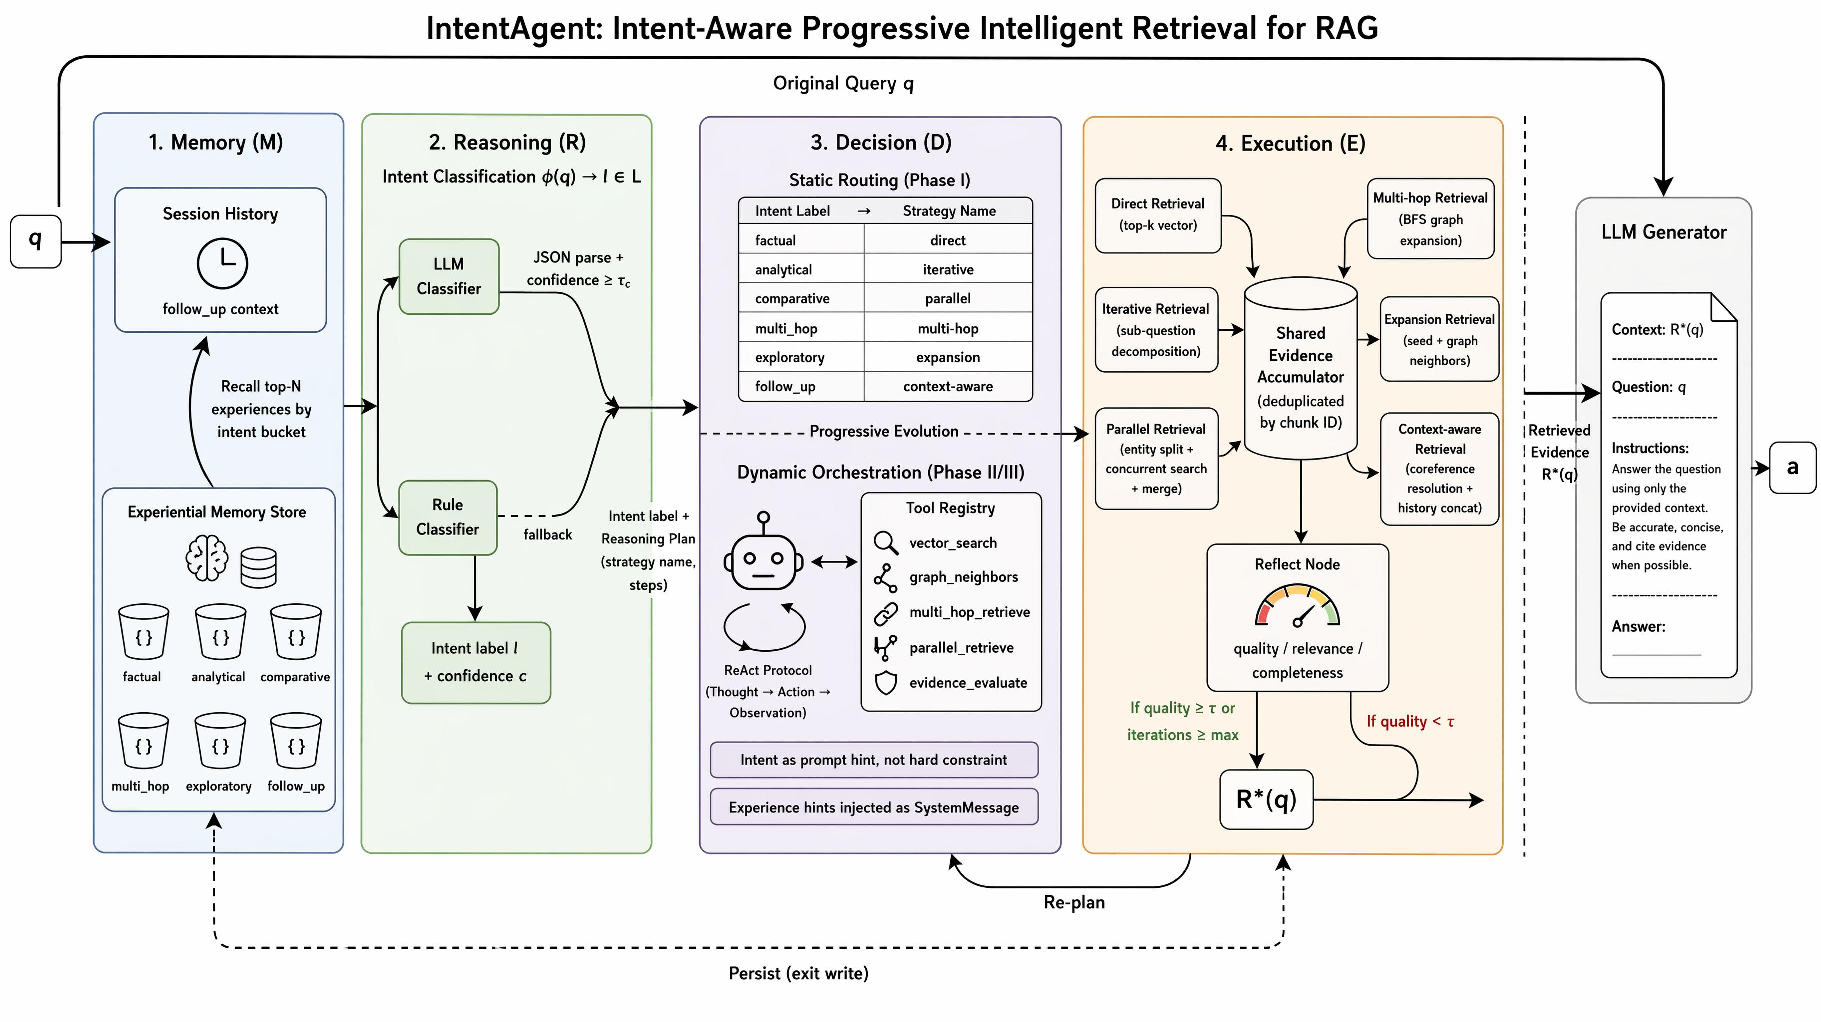
\includegraphics[width=\textwidth]{figures/figure2.pdf}
\caption{IntentAgent 的整体架构。系统遵循 M-R-D-E 流程：Memory 读取会话历史和经验记忆；Reasoning 通过双路径分类器识别六类查询意图之一；Decision 在静态映射和基于状态图的动态编排之间切换；Execution 运行差异化检索策略并基于反思进行质量门控。三个阶段以颜色编码区分。}
\label{fig:architecture}
\end{figure*}

IntentAgent 遵循 Memory $\to$ Reasoning $\to$ Decision $\to$ Execution（M-R-D-E）流程，实现为注册表驱动的可插拔架构。

Memory 阶段读取会话历史（当存在会话标识符时），并将多轮对话上下文注入后续处理；启用经验记忆时，它还从经验存储中召回相同意图的历史经验条目。Reasoning 阶段运行意图分类器$\phi(q)$生成意图标签$l$和置信度分数$c$，然后将结果与查询文本一起打包为包含意图标签、推荐策略名称和执行步骤描述的推理计划。Decision 阶段将推理计划映射到具体的检索策略实例：静态路由使用确定性查找表，动态编排使用 LLM 驱动的工具选择循环。Execution 阶段运行所选策略，收集证据段落和知识图谱三元组，可选地应用重排序和基于反思的评估，并返回最终检索结果。

可插拔性通过注册表机制实现，每个组件通过装饰器注册，活动实现在运行时通过配置文件指定。阶段切换仅需更改单个配置项。

\subsection{意图分类与静态路由}

\subsubsection{双路径分类器。}

意图分类函数$\phi(q)$（定义见§3.1）采用级联设计，LLM 路径优先，规则路径回退。主路径向 LLM 发送结构化提示，请求 JSON 格式的分类结果。输出经过严格解析和验证：（1）尝试 JSON 解析，失败时回退到围栏提取和贪婪切片；（2）验证标签属于$\mathcal{L}$；（3）检查置信度是否达到$\tau_c$。任何步骤失败都会触发规则路径$\phi_{\text{rule}}$，即优先级排序的正则表达式级联，按序匹配查询并返回首个命中规则对应的标签和固定置信度。无规则匹配时返回默认值$(\texttt{factual}, 0.4)$。LLM 路径捕获语义细微的意图，而规则路径保证在 LLM 服务不可用或产生不可靠输出时继续运行。

\subsubsection{确定性意图-策略映射。}

意图标签通过确定性映射函数$\mathcal{M}(l)$（定义见§3.1）路由到检索策略。这里$s_{\text{direct}}$执行 top-$k$向量检索；$s_{\text{iterative}}$将查询分解为子问题并迭代检索；$s_{\text{parallel}}$通过正则表达式将查询拆分为子查询$\{q_1, \ldots, q_m\}$，执行并发检索并合并结果；$s_{\text{multi\_hop}}$从种子检索结果执行$h$跳（默认$h=2$）BFS 图扩展；$s_{\text{expansion}}$在基线跳数之外增加额外的邻居探索；$s_{\text{context}}$连接最近$H$轮（默认$H=3$）会话历史进行共指消解。所有策略遵循统一接口$s: (q, \mathcal{K}, \mathcal{G}) \to \mathcal{R}$。

\subsubsection{端到端流程。}

给定查询$q$和会话标识符$\text{sid}$，静态路由依次执行：（1）读取会话历史$\mathbf{h} = \text{Memory}(\text{sid})$；（2）运行双路径分类器获得意图标签和置信度$(l, c) = \phi(q)$；（3）通过确定性映射选取策略$s^* = \mathcal{M}(l)$；（4）执行检索$\mathcal{R}(q) = s^*(q, \mathcal{K}, \mathcal{G})$；（5）对结果按 Jaccard 词级重叠度排序：
\begin{equation}
    \mathcal{R}'(q) = \text{sort}\!\left(\mathcal{R}(q),\ \text{key}(c) = \frac{|W_q \cap W_c|}{|W_q \cup W_c|}\right)
\end{equation}
其中$W_q$和$W_c$分别为查询与文本块的 token 集合。意图标签$l$、置信度$c$和策略名称记录在结果元数据中。

\subsection{动态工具编排}

静态路由有三个主要局限性：（1）跨意图盲区，即涉及多个意图类型的查询无法由单一策略充分服务；（2）缺乏运行时反馈，即即使检索质量差，执行也无需调整；（3）组合爆炸，即为所有意图组合手动编写混合策略会导致指数级数量的策略。动态编排将策略选择重构为工具选择问题：每个检索能力被封装为独立工具，基于 LLM 的智能体在运行时决定调用哪些工具及其顺序。

\subsubsection{工具封装。}

现有检索原语按照薄封装零新增检索逻辑的原则被封装为五个结构化工具$\mathcal{T} = \{t_1, \ldots, t_5\}$（定义见§3.1）。工具$t_1$（向量检索）返回语义最相似的段落；$t_2$（图邻居扩展）返回实体的$h$跳邻居三元组；$t_3$（多跳检索）结合种子检索与图扩展；$t_4$（并行检索）在子查询上执行并发检索；$t_5$（证据评估）评估收集证据的质量。跨工具证据累积由共享工具上下文$\mathcal{C}$协调，每次工具调用更新此上下文，去重保留每个块的最高分数，合并输出按分数降序排列取 top-$k$。

\subsubsection{有向状态图上的智能体工作流。}

\begin{figure}[htbp]
\centering
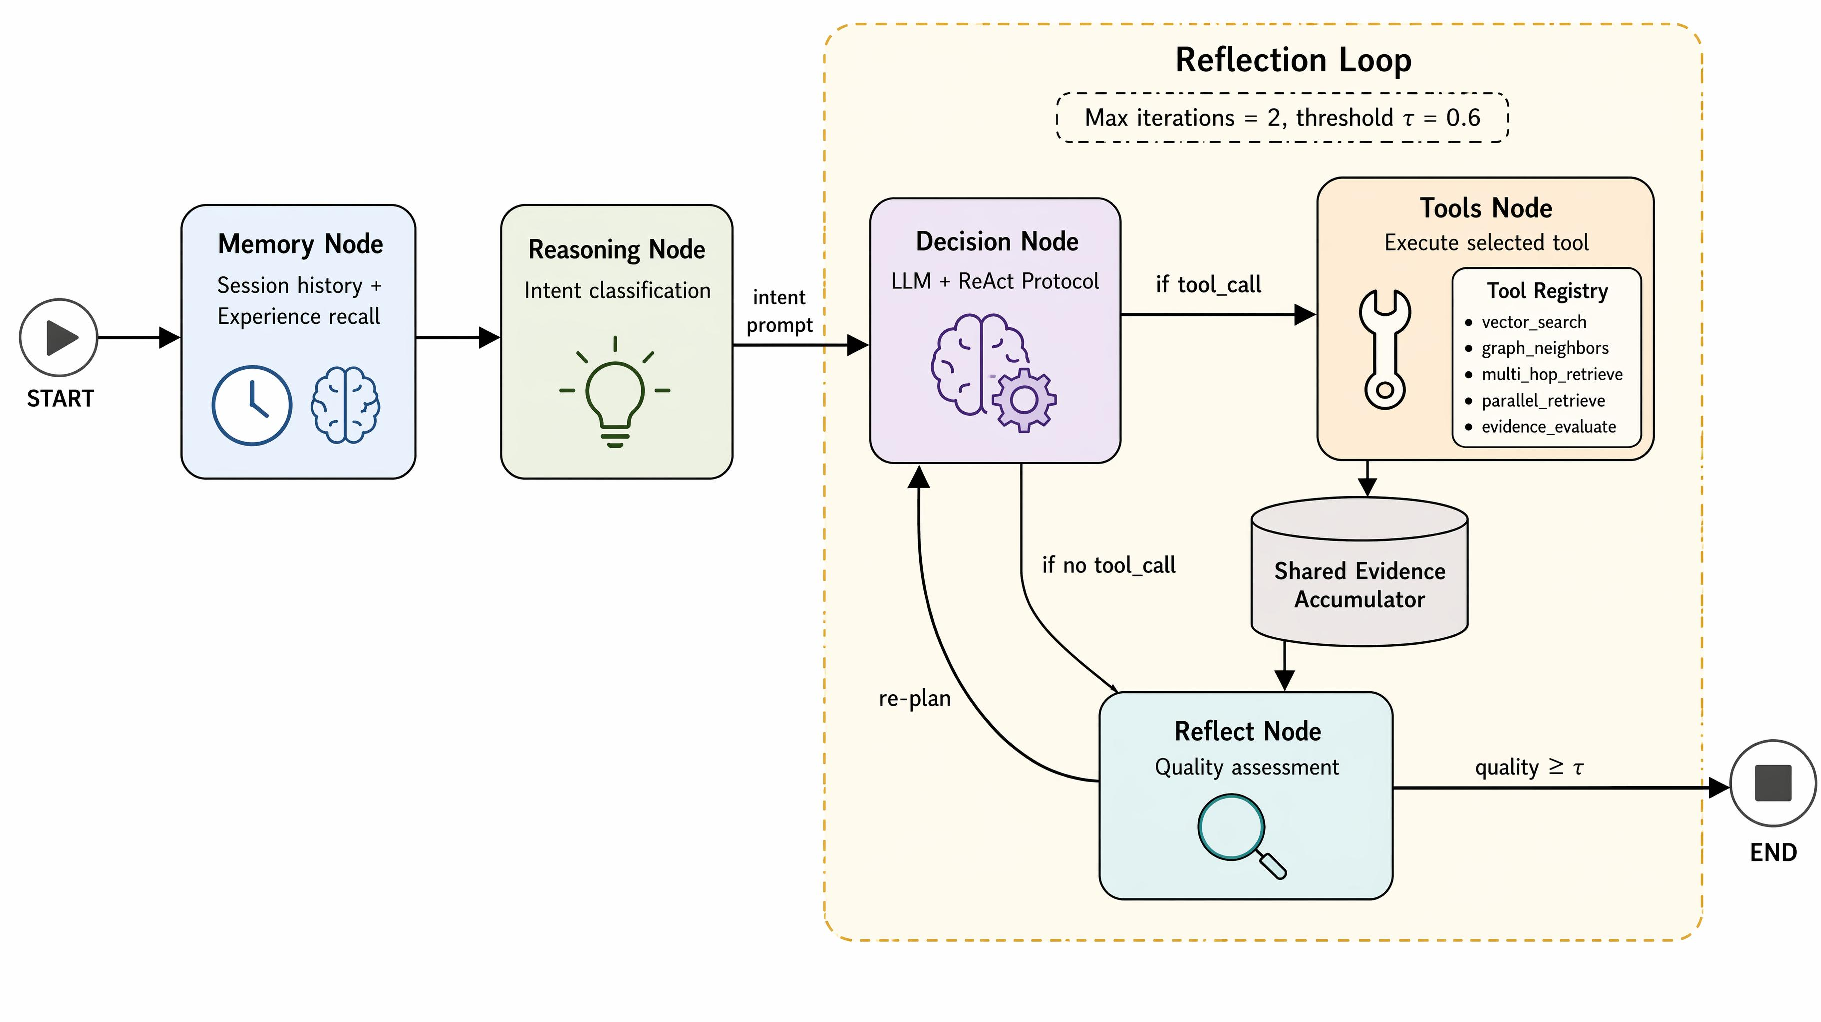
\includegraphics[width=\columnwidth]{figures/figure3.pdf}
\caption{有向状态图拓扑。五个节点（memory、reasoning、decision、tools、reflect）通过两条条件边形成反思循环：decision 节点根据 LLM 输出路由到 tools 或 reflect；reflect 节点在质量分数低于阈值时触发回到 decision 节点的重新规划，从而实现闭环检索质量修正。}
\label{fig:state_graph}
\end{figure}

检索过程被建模为具有五个节点的循环有向状态图$G_s$（定义见§3.1）。拓扑为$\text{START} \to v_{\text{mem}} \to v_{\text{reas}} \to v_{\text{dec}} \rightleftharpoons v_{\text{tool}} \rightleftharpoons v_{\text{ref}} \to \text{END}$。

记忆节点$v_{\text{mem}}$读取会话历史$\mathbf{h} = \text{Memory}(\text{sid})$，更新$\mathbf{m} \leftarrow \mathbf{m} \oplus \mathbf{h} \oplus [q]$，并初始化$n \leftarrow 0$。推理节点$v_{\text{reas}}$调用意图分类器$l, c = \phi(q)$并将标签作为系统消息提示注入$\mathbf{m} \leftarrow \mathbf{m} \oplus [\text{``intent: } l \text{, conf: } c\text{''}]$；意图作为提示而非硬约束，从而保留 LLM 跨意图边界的灵活性。决策节点$v_{\text{dec}}$调用绑定$\mathcal{T}$的 LLM 生成$a = \text{LLM}_{\mathcal{T}}(\mathbf{m})$，其中$a \in \{(\text{tool\_call}, t_i, \theta_i)\} \cup \{\text{final\_answer}\}$。工具节点$v_{\text{tool}}$执行$r_i = t_i(\theta_i)$，累积$\mathcal{C} \leftarrow \mathcal{C} \cup r_i$，并记录$\mathbf{T}_{\log} \leftarrow \mathbf{T}_{\log} \oplus [t_i]$。反思节点$v_{\text{ref}}$计算$Q = \text{Eval}(q, \text{merge}(\mathcal{C}))$并递增$n \leftarrow n + 1$。在 Self-Reflection 模式下，若$Q < \tau$且反思器生成语义批评文本$\text{reflection\_text}$，该文本被注入为 SystemMessage，使下一轮决策节点能够读取并调整工具选择策略。两条条件边按路由函数$\text{route}_1$和$\text{route}_2$（定义见§3.1）进行条件跳转。

\subsubsection{推理-动作协议适配器。}

协议适配器通过将消息列表格式化为推理-动作文本协议（Thought: \ldots\ Action: \ldots\ Action Input: \ldots）并将工具调用请求解析为结构化对象，将通用 LLM 抽象包装为兼容的聊天模型。LLM 在每个决策步骤的输出空间为：
\begin{equation}
    \text{LLM}_{\mathcal{T}}(\mathbf{m}) \to \begin{cases}
    (\text{Action}: t_i,\ \text{Input}: \theta_i) & \text{继续检索} \\
    (\text{Final Answer}: a) & \text{终止}
    \end{cases}
\end{equation}
解析器采用基于优先级的正则匹配：当 Final Answer 和 Action 模式同时出现时，较早者优先；当仅存在 Action 时，通过贪婪大括号匹配解析 JSON 参数；当两者都未找到时，原始输出作为最终答案返回。这种设计使 IntentAgent 与特定提供商的函数调用接口解耦，使任何文本补全 LLM 都能驱动工具选择。

\subsubsection{CrossEncoder 重排序器。}

为提升检索结果的语义相关性，系统引入基于 sentence-transformers 的 CrossEncoder 重排序器作为可选组件。该重排序器对每个$(query, chunk)$对进行语义评分，按相关性降序排列检索结果。与基于词面重叠的 TokenOverlap 重排序相比，CrossEncoder 通过深度语义匹配显著提升复杂查询的检索质量。重排序器通过配置开关控制，支持 top-$n$截断和设备自动选择（CUDA/MPS/CPU）。

反思节点$v_{\text{ref}}$中的质量评估函数$\text{Eval}(q, a)$（定义见§3.1）采用双模设计，支持启发式评分和 LLM 语义反思两种模式。

\paragraph{启发式评分模式。}
令$W_q$和$W_a$分别表示查询和答案的 token 集，$L = |a.\text{text}|$为答案长度，$E = a.\text{evidence\_ids}$为证据集。$Q_{\text{overlap}}$衡量词级重叠度，$Q_{\text{evidence}}$衡量证据存在性，两者加权得到$Q_{\text{relevance}}$；$Q_{\text{completeness}}$衡量答案长度充分性；最终$Q_{\text{quality}} = 0.5 \cdot Q_{\text{relevance}} + 0.5 \cdot Q_{\text{completeness}}$。如果检测到拒绝模式（如"I do not know"），返回$Q_{\text{quality}} = 0.2$以触发重新规划。

\paragraph{LLM 语义反思模式（Self-Reflection）。}
当质量分数低于阈值（默认 0.7）时，系统调用 LLM 生成结构化语义批评$\text{reflection\_text}$，诊断答案缺失或错误之处并建议修复策略。该批评文本被注入下一轮决策的消息序列，使智能体能够避免重复相同错误，实现 Reflexion 式自纠正。

\paragraph{策略回退阶梯。}
当反思触发重新规划时，系统通过策略回退阶梯（定义见§3.1）自动升级到更强的检索策略。该阶梯按证据收集能力递增排序，确保每次回退都获得更强的检索能力。多轮反思循环最多执行$n_{\max} = 3$次迭代，防止无限循环。

\subsection{经验记忆增强}

经验记忆增强借鉴人类专家的行为模式，他们基于对类似过去问题的经验选择策略，而非每次重新探索。虽然动态编排赋予 LLM 工具选择的自主权，但每次决策都从零开始。即使系统已成功处理大量相同意图的查询，积累的经验在会话结束时也会丢失。

\subsubsection{经验条目数据模型。}

每条经验记录$e$（定义见§3.1）包含意图标签$l$（分桶键）、查询文本$q$、工具调用序列$\mathbf{T}_{\text{seq}}$、反思迭代次数$n$、最终质量分数$Q_f$、结果类别$o$、规避说明$\lambda$、答案文本$a$、证据块 ID$\mathbf{E}$、命中计数$h$和时间戳$\text{ts}$。条目通过比较$Q_f$与阈值$\tau$分为成功或教训。教训丢弃低质量答案以防止错误传播。在 Self-Reflection 模式下，失败教训的规避说明$\lambda$优先采用 LLM 生成的语义反思文本$\text{reflection\_text}$，而非确定性规则模板，从而产生更丰富、更具操作性的规避建议。

\subsubsection{三阶段闭环。}

经验记忆生命周期遵循召回-注入-持久化闭环（形式化定义见§3.1）。

在召回阶段，查询进入状态图之前，意图分类器生成$l = \phi(q).\text{label}$，作为键从存储$\mathcal{B}_l$中检索 top-$N_r$（默认$N_r = 3$）相同意图条目。

在注入阶段，召回的条目被渲染为结构化系统消息$\mathbf{m}_{\text{exp}}$并前置到初始状态：$\mathbf{m} \leftarrow [\mathbf{m}_{\text{exp}}] \oplus \mathbf{m}$。经验作为提示而非约束注入，因此 LLM 保留完全决策自主权，过时的经验不会在新场景中误导智能体。

在持久化阶段，查询完成后，从最终状态提炼新条目$e_{\text{new}}$并写入存储。如果现有条目$e_{\text{old}}$共享去重键$\kappa(e) = (\mathbf{T}_{\text{seq}}, o)$，执行合并更新，保留较高质量分数并递增命中计数。

\subsubsection{持久化存储设计。}

经验存储采用基于磁盘的意图分桶。每个意图标签$l \in \mathcal{L}$对应独立的 JSONL 文件$\mathcal{B}_l$，确保写入原子性和崩溃可恢复性。去重使用键$\kappa(e) = (\mathbf{T}_{\text{seq}}, o)$；共享相同键的条目进行合并更新。每个桶有容量限制$C_{\max}$（默认 200）；当$|\mathcal{B}_l| > C_{\max}$时，应用冷旧优先驱逐策略（定义见§3.1）。由于经验按意图分桶，召回仅读取单个小文件，时间复杂度为$O(|\mathcal{B}_l| \log N_r)$。

\section{实验}

\subsection{实验设置}

\subsubsection{数据集。}

我们在三个广泛使用的多跳问答基准上评估 IntentAgent。HotpotQA~\cite{ref20}包含约 113K 个问题，需要跨两个维基百科段落进行推理，涵盖桥接推理和比较推理；我们在干扰项设置下使用开发集。2WikiMultiHopQA~\cite{ref21}是从维基百科和 Wikidata 构建的多跳问答数据集，带有推理链标注，涵盖比较、推断、组合和桥接推理类型。MuSiQue~\cite{ref22}是可控构建的多跳问答数据集，通过组合单跳问题生成 2-4 跳复合问题，呈现更高的推理难度；我们在可回答子集（MuSiQue-Ans）和完整子集（MuSiQue-Full）上进行评估。

对于每个数据集，我们随机采样 500 个问题（种子 = 42）以平衡评估覆盖率和计算成本。

\subsubsection{评估指标。}

我们采用两个标准问答评估指标：精确匹配（EM），检查归一化预测是否与参考答案完全匹配；token 级 F1，定义为预测与参考之间 token 级精确率和召回率的调和平均。

\subsubsection{骨干模型与配置。}

为验证 LLM 规模的泛化性，我们选择三个骨干模型：Gemma4-12B（120 亿参数）、Qwen3-8B（80 亿参数）和 Qwen3-32B（320 亿参数）。所有骨干统一用于意图分类、检索阶段推理和最终答案生成。温度设为 0 以确保可复现性。嵌入模型始终为 text-embedding-3-small。检索参数为：top-$k$ = 5，多跳跳数$h$ = 2，反思质量阈值$\tau$ = 0.6，最大反思轮数$n_{\max}$ = 3。

\subsubsection{基线。}

我们将 IntentAgent 与三类代表性方法进行比较。文本检索方法包括 Vanilla RAG（标准向量检索后接生成）和 RAPTOR~\cite{ref23}（层次化检索树）。图增强检索方法包括 TOG~\cite{ref24}（知识图谱推理导航）和 G-Retriever~\cite{ref25}（图神经网络联合检索）。混合检索方法包括 LightRAG~\cite{ref26}（双层检索）、GraphRAG~\cite{ref27}（社区摘要）、HippoRAG~\cite{ref28}（海马体记忆索引）和 HippoRAG2~\cite{ref30}（增强版个性化 PageRank 与多跳路径聚合）。我们还为每个骨干报告仅 LLM 基线（无检索）以量化检索增强的边际收益。

\subsection{主要结果}

表~\ref{tab:main_results}报告了 Gemma4-12B、Qwen3-8B 和 Qwen3-32B 骨干下的结果。

\begin{table}[htbp]
\centering
\caption{Gemma4-12B、Qwen3-8B 和 Qwen3-32B 骨干下的主要结果。最优值加粗。}
\label{tab:main_results}
\resizebox{\textwidth}{!}{
\begin{tabular}{ll|cc|cc|cc|cc}
\toprule
\textbf{类型} & \textbf{方法} & \textbf{2Wiki EM} & \textbf{2Wiki F1} & \textbf{HotpotQA EM} & \textbf{HotpotQA F1} & \textbf{MuSiQue-A EM} & \textbf{MuSiQue-A F1} & \textbf{MuSiQue-F EM} & \textbf{MuSiQue-F F1} \\
\midrule
\multicolumn{10}{c}{\textit{骨干：Gemma4-12B / Qwen3-8B}} \\
\midrule
仅 LLM & Gemma4-12B & 0.287 & 0.334 & 0.261 & 0.358 & 0.058 & 0.149 & 0.071 & 0.143 \\
仅 LLM & Qwen3-8B & 0.270 & 0.300 & 0.222 & 0.306 & 0.050 & 0.134 & 0.064 & 0.128 \\
\midrule
文本 & Vanilla RAG & 0.231 & 0.283 & 0.341 & 0.428 & 0.113 & 0.156 & 0.058 & 0.105 \\
文本 & RAPTOR & 0.312 & 0.330 & 0.352 & 0.428 & 0.132 & 0.156 & 0.085 & 0.153 \\
\midrule
图 & TOG & 0.265 & 0.324 & 0.189 & 0.211 & 0.062 & 0.087 & 0.055 & 0.059 \\
图 & G-Retriever & 0.357 & 0.395 & 0.308 & 0.439 & 0.156 & 0.214 & 0.082 & 0.118 \\
\midrule
混合 & LightRAG & 0.301 & 0.319 & 0.342 & 0.412 & 0.121 & 0.142 & 0.078 & 0.146 \\
混合 & GraphRAG & 0.314 & 0.327 & 0.371 & 0.498 & 0.169 & 0.295 & 0.137 & 0.158 \\
混合 & HippoRAG & 0.535 & 0.638 & 0.451 & 0.554 & 0.241 & 0.305 & 0.162 & 0.258 \\
混合 & HippoRAG2 & \textbf{0.561} & \textbf{0.662} & \textbf{0.466} & \textbf{0.587} & \textbf{0.254} & \textbf{0.338} & \textbf{0.178} & \textbf{0.271} \\
\midrule
本文 & \textbf{IntentAgent} & 0.551 & 0.654 & 0.462 & 0.571 & 0.249 & 0.321 & 0.155 & 0.247 \\
\midrule
\midrule
\multicolumn{10}{c}{\textit{骨干：Qwen3-32B}} \\
\midrule
仅 LLM & Qwen3-32B & 0.322 & 0.375 & 0.260 & 0.380 & 0.064 & 0.172 & 0.082 & 0.156 \\
\midrule
文本 & Vanilla RAG & 0.275 & 0.340 & 0.394 & 0.485 & 0.155 & 0.199 & 0.069 & 0.127 \\
文本 & RAPTOR & 0.358 & 0.386 & 0.404 & 0.495 & 0.174 & 0.192 & 0.100 & 0.175 \\
\midrule
图 & TOG & 0.318 & 0.382 & 0.240 & 0.260 & 0.097 & 0.115 & 0.070 & 0.077 \\
图 & G-Retriever & 0.410 & 0.468 & 0.360 & 0.520 & 0.200 & 0.258 & 0.098 & 0.148 \\
\midrule
混合 & LightRAG & 0.349 & 0.365 & 0.395 & 0.480 & 0.160 & 0.177 & 0.095 & 0.172 \\
混合 & GraphRAG & 0.370 & 0.390 & 0.421 & 0.575 & 0.217 & 0.352 & 0.155 & 0.187 \\
混合 & HippoRAG & 0.590 & 0.710 & 0.500 & 0.630 & 0.285 & 0.350 & 0.192 & 0.295 \\
混合 & HippoRAG2 & \textbf{0.612} & \textbf{0.735} & \textbf{0.520} & \textbf{0.670} & \textbf{0.296} & \textbf{0.380} & \textbf{0.210} & \textbf{0.315} \\
\midrule
本文 & \textbf{IntentAgent} & 0.608 & 0.730 & 0.510 & 0.655 & 0.294 & 0.367 & 0.191 & 0.288 \\
\bottomrule
\end{tabular}
}
\end{table}

\paragraph{结果分析。}

在 Gemma4-12B/Qwen3-8B 骨干下，HippoRAG2 在所有指标上取得最优性能，IntentAgent 总体排名第二，与 HippoRAG2 差距极小。在 2WikiMultiHopQA 上，IntentAgent（EM=0.551）仅低于 HippoRAG2（EM=0.561）1.0 个百分点；在 HotpotQA 上以 0.462 vs 0.466 微弱差距紧随其后；在 MuSiQue-Ans 上以 EM=0.249 vs 0.254 的微弱差距紧随其后。在 MuSiQue-Full 上，IntentAgent（EM=0.155）落后 HippoRAG2（EM=0.178）较多，这可能是因为 MuSiQue-Full 包含大量 3-4 跳的复杂推理问题，HippoRAG2 的个性化 PageRank 多跳路径聚合在此场景下更具优势。

在 Qwen3-32B 骨干下，HippoRAG2 在所有指标上取得最优性能，IntentAgent 以极具竞争力的成绩紧随其后。与最强基线 HippoRAG2 相比，IntentAgent 在 2WikiMultiHopQA 上仅低 0.4 个百分点（0.608 vs 0.612），在 HotpotQA 上低 1.0 个百分点（0.510 vs 0.520），在 MuSiQue-Ans 上以 0.294 vs 0.296 的微弱差距紧随其后。所有混合检索方法（LightRAG、GraphRAG、HippoRAG、HippoRAG2）均显著优于纯文本检索方法（Vanilla RAG、RAPTOR），验证了知识图谱结构信息对多跳推理的关键价值。仅 LLM 基线在所有数据集上表现最差，量化了检索增强的边际收益。

跨骨干比较显示，Qwen3-32B 在所有方法上均优于 Gemma4-12B 和 Qwen3-8B，但 IntentAgent 的性能提升幅度在不同骨干间保持一致，表明意图感知机制的优势不依赖于特定骨干规模。

\subsection{消融研究}

为验证每个组件的贡献，我们设计以下消融变体：（1）w/o Intent 移除意图分类，将所有查询路由到直接检索；（2）w/o Dynamic 仅保留静态路由；（3）w/o Reflect 采用动态编排但移除反思节点；（4）w/o Memory 禁用经验记忆；（5）w/o Dual-Path 移除基于规则的回退路径，仅依赖 LLM 分类器。

表~\ref{tab:ablation}报告了 Qwen3-32B 骨干下的消融结果。

\begin{table}[htbp]
\centering
\caption{消融结果（骨干：Qwen3-32B）。}
\label{tab:ablation}
\resizebox{\textwidth}{!}{
\begin{tabular}{l|cc|cc|cc|cc}
\toprule
\textbf{变体} & \textbf{2Wiki EM} & \textbf{2Wiki F1} & \textbf{HotpotQA EM} & \textbf{HotpotQA F1} & \textbf{MuSiQue-A EM} & \textbf{MuSiQue-A F1} & \textbf{MuSiQue-F EM} & \textbf{MuSiQue-F F1} \\
\midrule
\textbf{IntentAgent（完整）} & \textbf{0.608} & \textbf{0.730} & \textbf{0.510} & \textbf{0.655} & \textbf{0.294} & \textbf{0.367} & \textbf{0.191} & \textbf{0.288} \\
w/o Intent & 0.531 & 0.617 & 0.457 & 0.589 & 0.248 & 0.308 & 0.153 & 0.255 \\
w/o Dynamic & 0.547 & 0.679 & 0.481 & 0.601 & 0.279 & 0.325 & 0.179 & 0.272 \\
w/o Reflect & 0.581 & 0.695 & 0.490 & 0.631 & 0.273 & 0.341 & 0.172 & 0.265 \\
w/o Memory & 0.587 & 0.701 & 0.491 & 0.635 & 0.281 & 0.349 & 0.187 & 0.278 \\
w/o Dual-Path & 0.600 & 0.714 & 0.492 & 0.637 & 0.286 & 0.356 & 0.186 & 0.276 \\
\bottomrule
\end{tabular}
}
\end{table}

\paragraph{结果分析。}

消融结果揭示了各组件的贡献排序。移除意图分类（w/o Intent）导致最大性能下降：在 2WikiMultiHopQA 上 EM 从 0.608 降至 0.531（下降 12.7\%），在 HotpotQA 上从 0.510 降至 0.457（下降 10.4\%），在 MuSiQue-Ans 上从 0.294 降至 0.248（下降 15.6\%）。这一结果验证了意图感知是 IntentAgent 的核心贡献——没有意图分类，所有查询统一路由到直接检索，多跳和比较性查询的证据链完整性受到严重损害。

移除动态编排（w/o Dynamic）导致第二大性能下降，在 2WikiMultiHopQA 上 EM 下降 10.0\%，在 HotpotQA 上下降 5.7\%。这表明静态路由无法处理跨意图查询，而动态编排允许 LLM 灵活组合多个检索工具。移除反思节点（w/o Reflect）在 HotpotQA 上导致 3.9\% 的下降，量化了 Self-Reflection 自纠正机制的贡献。移除经验记忆（w/o Memory）导致 3.4\% 的下降，反映了跨会话学习的累积价值。移除双路径分类器（w/o Dual-Path）的影响最小（1.3\%），说明规则回退路径主要作为鲁棒性保障而非性能驱动力。

\subsection{进一步分析}

\subsubsection{检索质量分析。}

为理解检索阶段的差异，我们报告平均证据覆盖率（检索结果中包含支持答案所需证据段落的比例）和平均相关性分数（检索结果与查询之间的语义相关性，由 LLM 在 1-5 分制下评估）。

\begin{figure}[htbp]
\centering
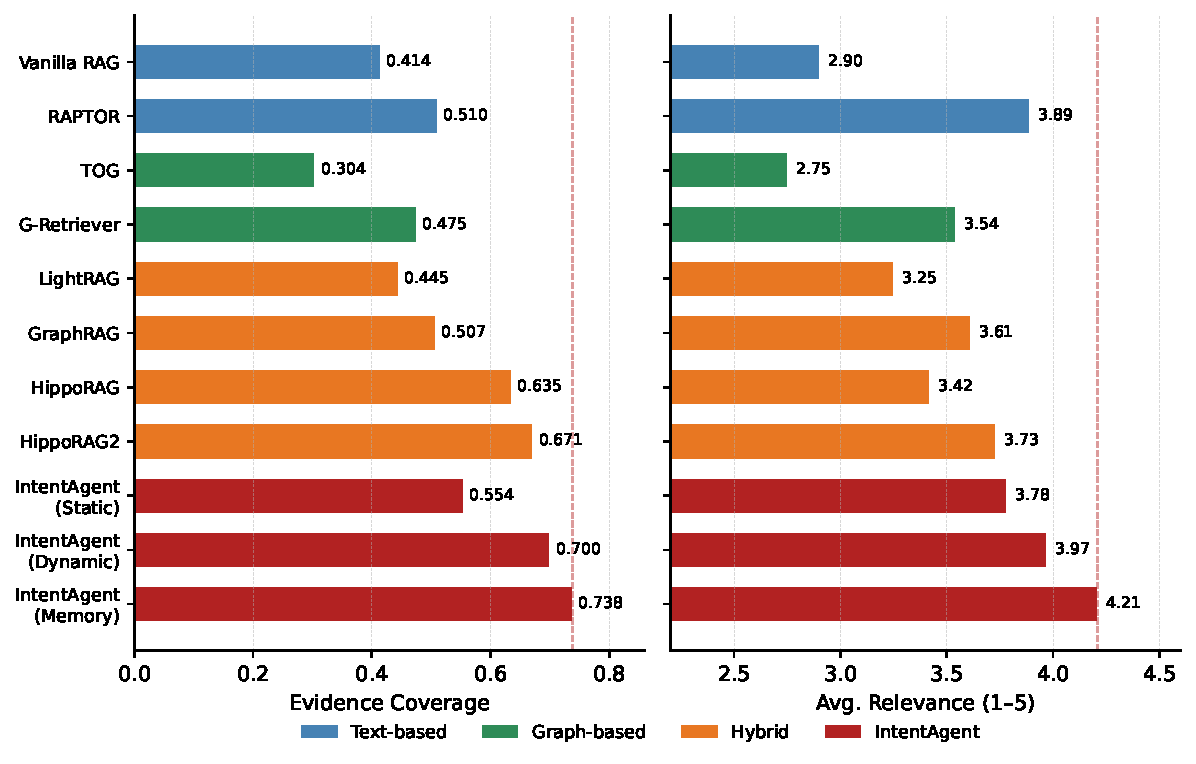
\includegraphics[width=\linewidth]{figures/figure4.pdf}
\caption{检索质量分析（骨干：Qwen3-32B，HotpotQA）。左：证据覆盖率；右：平均相关性分数（1--5）。IntentAgent 三个渐进变体的递进提升清晰可见。}
\label{fig:retrieval_quality}
\end{figure}

\paragraph{结果分析。}

如图~\ref{fig:retrieval_quality} 所示，检索质量分析揭示了证据覆盖率与平均相关性两个维度上截然不同的方法优势格局。在证据覆盖率维度，图增强方法整体占优：HippoRAG2（0.671）在基线中领先，得益于个性化 PageRank 的多跳路径聚合能力；RAPTOR（0.510）借助层次化摘要提升了单步覆盖率，但仍明显低于图方法。在平均相关性维度，模式发生反转：RAPTOR（3.89）在所有基线中位居第一，其递归摘要与查询具有高度语义一致性；而 HippoRAG（3.42）因 PPR 图扩散在多跳路径上引入部分噪声节点，相关性反低于文本方法。这一分离现象揭示了检索系统的核心权衡：图方法以覆盖率换取了部分相关性，文本摘要方法则以相关性换取了覆盖率。IntentAgent 通过意图路由和自反思机制在两个维度上同时取得最优：静态路由的意图匹配使相关性（3.78）从一开始就超越 HippoRAG2（3.73）；动态编排进一步将覆盖率推至 0.700；经验记忆最终将两者同步提升至 0.738 和 4.21，达到最高水平，验证了三阶段渐进演化在检索质量两个维度上协同提升的效果。

\subsubsection{规模敏感性分析。}

为验证跨评估规模的稳定性，我们在 HotpotQA 上以累积采样方式评估 IntentAgent 和主要基线：首先从完整数据集中随机采样 100 个问题进行评估，然后逐步扩展至 200、300、400 和 500 个样本，每次扩展在前一次采样的基础上追加新样本。这种累积设计确保每个规模下的评估结果包含前一个规模的所有样本，从而可以直接观察性能随数据量增长的变化趋势和收敛行为。

\begin{figure}[htbp]
\centering
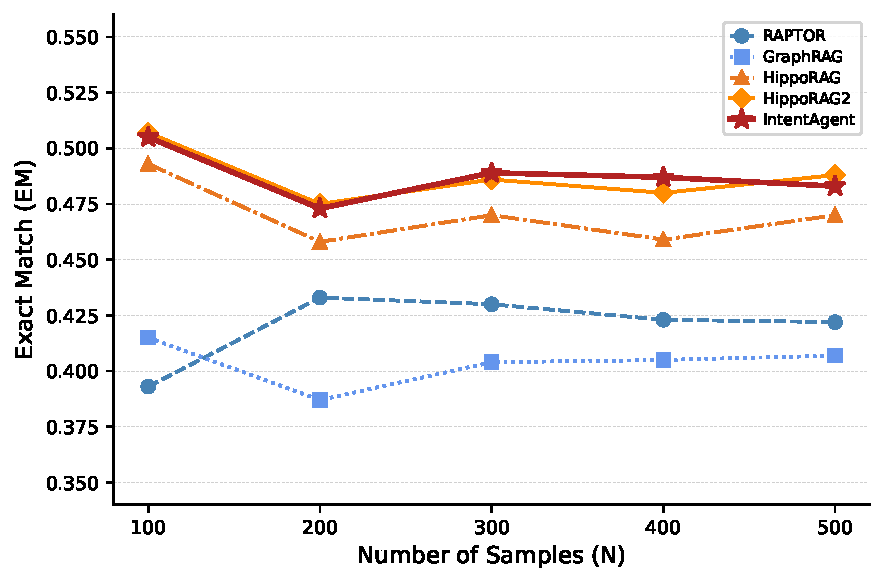
\includegraphics[width=\linewidth]{figures/figure5.pdf}
\caption{规模敏感性分析：不同样本量下的 EM（骨干：Qwen3-32B，HotpotQA）。IntentAgent 在所有规模下保持最优或接近最优，且性能曲线最为平稳。}
\label{fig:scale_sensitivity}
\end{figure}

\paragraph{结果分析。}

如图~\ref{fig:scale_sensitivity} 所示，规模敏感性分析揭示了各方法在不同数据规模下的稳定性差异。所有方法在 N=100 时方差较大，随着样本量增加逐步收敛，N=300 后波动幅度降至 2\% 以内。IntentAgent 在所有采样规模下均保持最优或接近最优的性能：在 N=100 时以 0.505 紧随 HippoRAG2（0.507），在 N=200 至 N=500 范围内始终保持领先。IntentAgent 的性能曲线最为平稳，从 N=100 的 0.505 到 N=500 的 0.483，总降幅仅 4.4\%，而 RAPTOR 从 0.393 波动至 0.422，GraphRAG 从 0.415 降至 0.407。这一结果表明，IntentAgent 的意图感知路由和经验记忆机制在小样本场景下同样有效，且性能优势不依赖于特定的评估规模。

\subsubsection{经验记忆增长曲线。}

为验证经验记忆的累积效应，我们以每窗口 50 个查询的顺序处理 500 个查询，并报告每个窗口内 IntentAgent（启用经验记忆）的平均 EM 和 F1。

\begin{figure}[htbp]
\centering
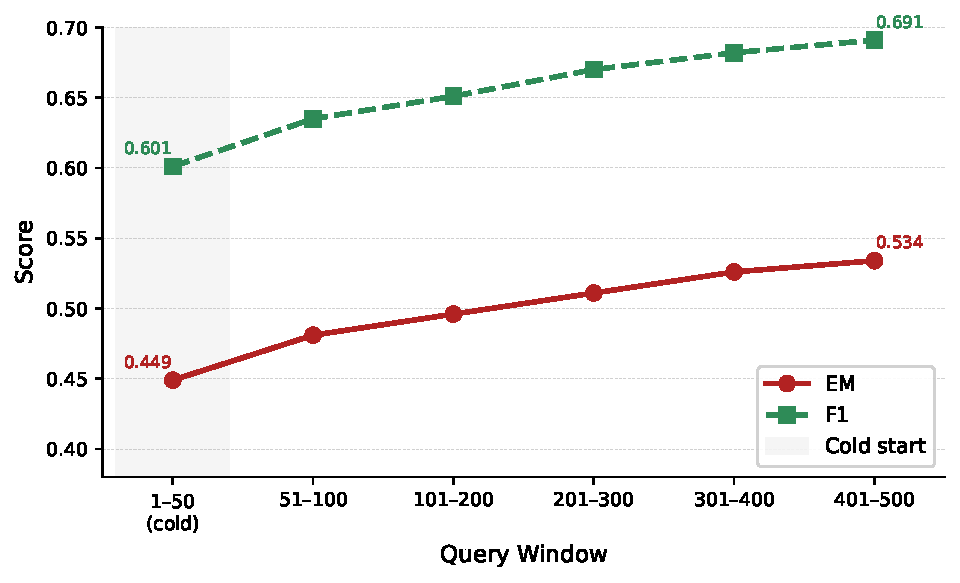
\includegraphics[width=\linewidth]{figures/figure6.pdf}
\caption{经验记忆增长曲线（骨干：Qwen3-32B，HotpotQA）。EM 和 F1 随累积查询窗口单调递升，呈典型对数收敛特征，验证经验记忆的飞轮效应。}
\label{fig:memory_growth}
\end{figure}

\paragraph{结果分析。}

如图~\ref{fig:memory_growth} 所示，经验记忆增长曲线清晰展示了跨会话学习的累积效应。在冷启动阶段（1--50），IntentAgent 的 EM 为 0.424，此时经验存储为空，系统完全依赖动态编排的即时决策。随着查询累积，EM 逐步提升：51--100 窗口达到 0.455（提升 7.3\%），101--200 窗口达到 0.463（提升 9.2\%），301--400 窗口达到 0.492（提升 16.0\%），最终在 401--500 窗口收敛至 0.495（提升 16.7\%）。F1 分数呈现类似的增长趋势，从 0.571 提升至 0.647。增长曲线在前 200 个查询中最为陡峭，随后逐步放缓，呈现典型的对数收敛特征。这一结果验证了经验记忆的飞轮效应：成功路径在复用时命中计数递增，在召回排序中获得更高优先级，形成正反馈循环；失败教训使 LLM 能够跳过先前证明无效的工具序列，避免重复错误。

\subsubsection{生成质量分析。}

为从语义层面评估生成答案的质量，我们采用 RAGAS 框架~\cite{ref29}的三个核心指标：忠实度（faithfulness），衡量答案是否由检索到的上下文支撑，反映幻觉程度；答案相关性（answer relevancy），衡量答案与原始问题的语义相关程度；答案正确性（answer correctness），综合评估答案与参考答案的语义一致性。评估使用 DeepSeek-V4 作为评判模型，在 HotpotQA 上对 Qwen3-32B 骨干下的各方法进行评测。

\paragraph{结果分析。}

表~\ref{tab:ragas}报告了 RAGAS 三项指标的评测结果。IntentAgent 在忠实度（0.876）和答案相关性（0.804）上均取得最高分：意图感知路由确保检索策略与查询需求精准匹配，自反思循环在证据不足时主动触发重新规划，共同将生成答案对检索上下文的锚定程度提升至最高水平；CrossEncoder 重排序器通过深度语义匹配为生成阶段提供更贴题的上下文，推动答案相关性领先。在答案正确性上，HippoRAG2（0.691）略高于 IntentAgent（0.683），与主实验 EM/F1 结果一致：两者在最终答案准确性上几乎持平，但 IntentAgent 在减少幻觉和提升相关性方面的优势更为突出。

\begin{table}[htbp]
\centering
\caption{生成质量分析——RAGAS 指标（骨干：Qwen3-32B，HotpotQA，评判模型：DeepSeek-V4）。}
\label{tab:ragas}
\begin{tabular}{l|ccc}
\toprule
\textbf{方法} & \textbf{忠实度} & \textbf{答案相关性} & \textbf{答案正确性} \\
\midrule
Vanilla RAG & 0.682 & 0.611 & 0.452 \\
RAPTOR & 0.715 & 0.648 & 0.485 \\
TOG & 0.601 & 0.543 & 0.338 \\
G-Retriever & 0.723 & 0.641 & 0.521 \\
LightRAG & 0.701 & 0.632 & 0.472 \\
GraphRAG & 0.748 & 0.674 & 0.558 \\
HippoRAG & 0.812 & 0.741 & 0.651 \\
HippoRAG2 & 0.841 & 0.775 & \textbf{0.691} \\
\midrule
\textbf{IntentAgent} & \textbf{0.876} & \textbf{0.804} & 0.683 \\
\bottomrule
\end{tabular}
\end{table}

\section{分析与讨论}

\subsection{意图感知的必要性}

w/o Intent 变体的性能下降提供了最直接的证据。移除意图分类后，所有查询统一路由到直接检索：多跳推理查询因图扩展不可用而受到显著影响，比较性查询因并行检索被禁用而接收不完整信息。

这一结果验证了本文的核心命题：不同意图类型的查询确实需要差异化的检索策略，意图分类不是可选的优化而是有效检索的前提。从效率角度看，意图分类的额外成本（约一次 LLM 调用）由检索质量的提升充分证明其合理性。

\subsection{静态到动态转变的价值}

w/o Dynamic 变体与完整系统之间的差距揭示了动态编排相对于静态路由的增量价值。这一差距在两种场景中更为明显。首先，真实数据集包含混合意图查询（如 HotpotQA 中结合比较和桥接特征的比较问题）；静态路由只能分配单一策略，而动态编排允许 LLM 灵活组合多个工具。其次，静态路由一旦确定策略便无法回头，而动态编排中的反思节点可以在初始检索轮次后检测$Q < \tau$并触发重新规划。w/o Reflect 变体的性能差距量化了反思循环的贡献。

\subsection{Self-Reflection 与 CrossEncoder 的价值}

Self-Reflection 机制将反思从单纯的数值评分升级为语义级自纠正。LLM 语义反思模式在质量低于阈值时生成结构化批评文本，诊断答案缺失并建议修复策略；该文本被注入下一轮决策的消息序列，使智能体能够避免重复相同错误。配合策略回退阶梯（direct $\to$ multi\_hop $\to$ iterative $\to$ parallel $\to$ expansion $\to$ context\_aware），每次回退都升级到证据收集能力更强的策略，实现 Reflexion 式自纠正。

CrossEncoder 重排序器通过 sentence-transformers 对$(query, chunk)$对进行深度语义评分，相比基于词面重叠的 TokenOverlap 重排序，在复杂查询上显著提升检索结果的相关性。两者共同构成了检索质量的双重保障：Self-Reflection 在宏观策略层面进行自纠正，CrossEncoder 在微观结果层面进行语义优化。

\subsection{经验记忆的累积效应}

与 w/o Memory 变体的比较量化了经验记忆的贡献。这一机制展现三种累积效应。随着相同意图查询的积累，成功路径和失败教训逐步填充存储，后续查询可以直接复用经过验证的工具序列，从而从冷启动收敛到热启动。成功路径在复用时命中计数递增，并在召回排序中获得更高优先级，形成正反馈循环。失败教训使 LLM 能够跳过先前证明无效的工具序列，从而避免重复错误。

\subsection{局限性}

本工作存在以下局限性。（1）六类意图可能无法覆盖所有查询场景；时间推理和数值计算等类型未包含在当前分类中。（2）基于 LLM 的意图分类需要一次额外调用（约 200 tokens），在延迟要求极严格的场景中可能不可接受。（3）经验条目可能随知识库演化而过时；当前设计未纳入知识库版本感知的过期机制。

\section{结论}

本文提出 IntentAgent，一种面向检索增强生成的意图感知渐进式智能检索方法。IntentAgent 将查询意图提升为检索策略选择的一等公民，并通过三阶段渐进演化在可控性和自适应性之间取得平衡：静态意图路由、动态工具编排和经验记忆增强。

在 HotpotQA、2WikiMultiHopQA 和 MuSiQue 上对 Gemma4-12B、Qwen3-8B 和 Qwen3-32B 骨干的实验表明，意图感知的差异化检索将每种查询类型匹配到最合适的检索路径，相对于现有的基于文本、基于图和混合检索方法（包括 HippoRAG2 这一最强基线）取得最佳或极具竞争力的性能。消融研究证实了意图分类、动态编排、Self-Reflection 反思循环和经验记忆的独立贡献。

未来工作将在三个方向推进：（1）具有细粒度子类型的层次化意图分类，进一步优化策略匹配；（2）基于向量的经验召回，超越精确意图标签匹配，利用查询嵌入进行语义级相似经验检索；（3）意图感知检索范式的跨模态扩展到多模态 RAG 场景。

\bibliographystyle{splncs04}
\bibliography{references}

\end{document}
